%!TEX root = ../main.tex


\section{Group-based Acceleration}
\label{sec:group}

As discussed above, we can observe that in Section~\ref{subsec:one}, even with the most efficient imputation-in-the-loop  strategy, \ie  one tuple in  each iteration, the time complexity is  $O(KhnL^2)$, where $K$ is the size of the coreset, $h$ is the sample size, $L$ is a small constant and $n$ is the number of entire dataset. Therefore, obviously, the efficiency is dominated by $n$, which is still low when $n$ is large, and thus it  is necessary to further accelerate this process.

\noindent \textbf{Key observation.}   Recap that in Figure~\ref{fig:overviewSingle}, we can observe that  given a tuple $c$ in the coreset, the tuples in the origin full train set $\train$ represented by $c$ are likely to be  closer to each other than other tuples not represented by $c$.
Based on this observation, we propose to first group the full train set, and then compute the coreset based on the groups. This can achieve much acceleration because the number of groups is much smaller than $n$. 

At the following, we will theoretically and empirically show the group-based solution can accelerate the coreset selection process without sacrificing the effectiveness much.

%the acceleration can be achieved by clustering the 

\subsection{Group-based Solution Overview}

%\begin{figure}[t]
 %   \centering
  %  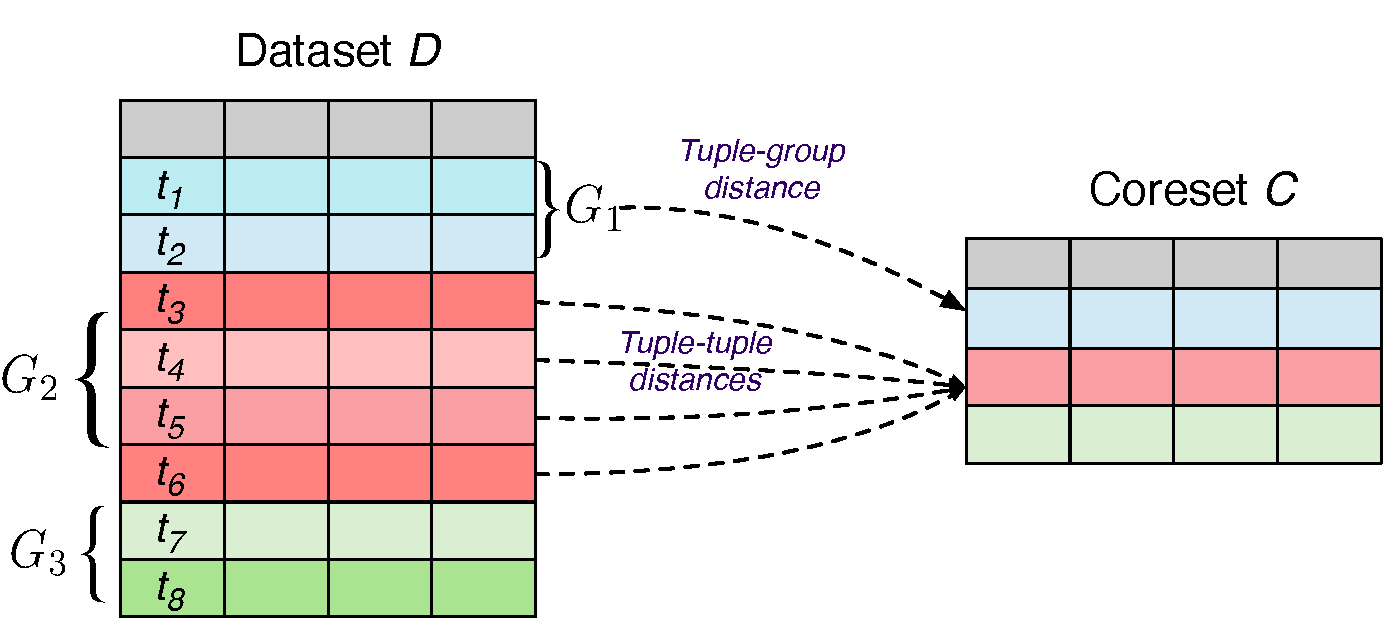
\includegraphics[width=0.6\textwidth]{figs/Overview-gb}
   % \vspace{-2.5em}
   % \caption{Illustration of the Group-based Solution.}
    %\label{fig:overview-gb}
   % \vspace{-1.5em}
%\end{figure}

%As shown in Figure~\ref{fig:overview-gb}, o
One of the core parts of coreset computation is to compute the tuple-tuple distance, \ie $s_{ij}$. For the group-based solution, we just need to consider the relationship between tuples and these pre-computed groups, namely tuple-group distance, rather than the large amount of tuple-tuple distances. As we will discuss below, the computation of tuple-group distance does not need to iterate all tuples in the group, and thus  the overall efficiency can be much improved. 

At a high level, the overall process of group-based \ours solution with imputation in the loop is shown in Algorithm~\ref{alg:group}. To be more explicit, we illustrate Algorithm~\ref{alg:group} in comparison with Algorithm~\ref{alg:framework} in Section~\ref{subsec:framework} without grouping (the modified parts are highlighted in blue fonts).

To be specific, as shown in Line~\ref{alg4:cluster}, we first group $\train$   using the efficient local sensitive hash (LSH) approach, where each group $\group_u, u\in[1, U]$ denotes the indexes of tuples in $\train$. In this way, every pair of tuples in the same group is close to each other in the feature distance.
%
 Afterwards, the major difference between group-based \ours and original \ours lies in the 3rd loop. Instead of  selecting a coreset to represent all tuples in the train set, group-based \ours selects a coreset to represent all clusters. As these clusters can well capture the train set distribution, the selected coreset contains enough information to approximate the full gradient of the entire train set. 
 
 To this end, recap that the typical coreset selection algorithm needs the tuple-tuple distances to approximate the full gradient, while for group-based \ours, we just need to consider the tuple-group distances, \ie  
$\overline{s}_{\gamma(j)u} = \max\limits_{v \in \group_u} s_{\gamma(j)v}, s_{\gamma(j)v} = \lVert\mathbf{x}_v - \mathbf{x}_{\gamma(j)}\rVert, \gamma(j)\in[1, n]$, which denotes the maximum feature distance between the tuple $c_j$ in the coreset and all tuples in $\group_u$. As tuples in $\group_u$ are close to each other, $\overline{s}_{\gamma(j)u}$ can represent the relationship between $c_j$ and tuples in $\group_u$ to a large extent.
%
We will theoretically show that using this maximum distance can still derive a bounded GA error. 
However, since computing $\overline{s}_{\gamma(j)u}$ needs to iterate the tuples in $\group_u$, which is time-consuming, we finally estimate an upper bound $\hat{s}_{ju}$ to compute the coreset score (as shown in Line~11), which still leads to a well-performed coreset. 
%

%!TEX root = ../main.tex

\begin{figure}[!t]
 \vspace{-1em}
	\begin{algorithm}[H]
		\normalem
	\caption{Group-based \ours Solution (imputation-in-the-loop) \label{alg:group}}
		{\small
			
		\KwIn{Incomplete train data $\train$, coreset size $\numcore$, sample size $h$.}
		
		\KwOut{A coreset $\core \subseteq \train$, weight $\weightset=\{w_j\}$,$|\core|=|\weightset|=\numcore$.}
		
		$C=\emptyset$;\\\nllabel{alg1:init1}
		
		\add{Cluster $\train$ into groups $\groups = \{ \group_1, \group_2, ..., \group_\groupsize \}$;}\\\nllabel{alg4:cluster}
		
		\While{$|\core|< \numcore$}
		{\nllabel{craig1:loop1}
			
		/*1st loop*/  \\
		
		Sample $h$ tuples as $T_{sample} \subseteq \train \setminus \core$\\\nllabel{craig1:sample}
		
			\For{each tuple $t \in T_{sample}$}  
			{\nllabel{craig1:loop2}
				
				/*2nd loop*/ \\
				 $\hat{\core} = \core \cup \{t\}$;\\
			%	}
			 %$\mathrm{E}[t|\core]=\texttt{ComputeUtility}(t, C,D)$;
				 %/*3rd loop*/  \\\nllabel{craig1:loop3}
				 \For{\add{each group $G_k \in \groups$}}  
				 {
				 	\add{/*3rd loop*/} \\
				 
				 	%	Get the possible worlds of $\hat{\core} \cup \{t_i\}$;\\\nllabel{one:enumw}
				 	%	Compute $\mathrm{E}[\min_{c_j\in \hat{\core}}s_{ij}]$ using these possible worlds and their probabilities;\\\nllabel{one:exp4pw}
				 		\add{$\mathrm{E}[\hat{\core}] +\!\!= \mathrm{E}[\min_{c_j\in \hat{\core}}\bound_{jk} \times |\group_k|]$, where $\bound_{jk}$ is the upper bound of} \\\quad \\\nllabel{alg4:bound} \add{$\overline{s}_{\gamma(j)k} = \max\limits_{v \in \group_k} s_{\gamma(j)v}, s_{\gamma(j)v} = \lVert\mathbf{x}_v - \mathbf{x}_{\gamma(j)}\rVert, \gamma(j)\in[1, n]$; }\\\nllabel{one:dirtysum}
			     }
		         \add{$\mathrm{E}[t|\core] = \mathrm{E}[\core] - \mathrm{E}[\hat{\core}];$}
				 
			}		

			$t^*$ = $\argmax_{t\in T_{sample}}\mathrm{E}[t|\core]$ ;\\\nllabel{craig1:maxmulti}
			\If{$\mathbb{I}[t^*] = 1$} {\nllabel{craig1:oracle1}
				        Impute $t$ by a  human or automatic method.\\\nllabel{craig1:oracle}
				    }
			$\core = \core \cup \{t^*\}$;
			\\\nllabel{craig1:add2} 
			
				%\If{$\mathbb{I}[t^*] = 1$}
		%	{ \nllabel{alg:if}
		%		 \cc{Impute $t^*$ (by human or automatic methods).}\\\nllabel{alg:oracle}
		%	
			%}					
		}
	 %   \For{ $t\in \core$} 
	  %  {\nllabel{craig1:goodcore1}
	 %      \If{$\mathbb{I}[t] = 1$} {\nllabel{craig1:oracle1}
	 %        Impute $t$ by a  human or automatic method.\\\nllabel{craig1:oracle}
      %       }
     %   }
    
	 	\For{$j = 1$ to $|\core|$} 
	 	{\nllabel{craig1:cc0}
	 		%$w_j = \sum_{i=1}^{n}\mathbb{I}'[j=\argmin_{c_{j'}\in\core}  %\max\limits_{\hypo\in\vartheta}\lVert \df_i(\hypo) - \df_{\gamma(j')}(\hypo) \rVert ]$;\\\nllabel{craig1:cc}
	 		\For{$i = 1$ to n}
	 		{
	 		  \If{$c_j=\argmin_{c_{j'}\in\core}\max\limits_{\hypo\in\vartheta}\lVert \df_i(\hypo) - \df_{\gamma(j')}(\hypo) \rVert$}
	 		  {
	 		  	$w_j~+\!=~1$;\\\nllabel{craig1:cc}
	 		  }
 		    }
	 		
	 	}
		\Return $\core,\weightset$;\\\nllabel{craig1:return}
		}
	\end{algorithm}
\end{figure}




\subsection{Group-based GA Error Bound}
\label{group-ea}

In this section, following the equations in previous sections, we deduce the GA error bound for our group-based solution. 
%
If we group $\train$ to $\{ \group_1 , \group_2, ...\group_U\}$, considering Equation~\ref{eqa:tuple}, we  can rewrite the sum of $n$ feature distances (\ie $\min_{c_j\in \core_k}\lVert\mathbf{x}_i - \mathbf{x}_{\gamma(j)}\rVert$) to $U$ summations as follows:

\begin{equation}\label{eqa:cluster-1}
    \mathrm{E}[C] = \sum_{k= 1}^{|\worlds|} p_k (\sum_{i=1}^n \min_{c_j\in C_k}\lVert\mathbf{x}_i - \mathbf{x}_{\gamma(j)}\rVert) =  \sum_{k= 1}^{|\worlds|} p_k (\sum_{u=1}^U\sum_{v \in \group_u} \min_{c_j\in C_k}\lVert\mathbf{x}_v - \mathbf{x}_{\gamma(j)}\rVert)
\end{equation}

Afterwards, each summation is the sum of $U$ feature distances, as shown in Equation~\ref{eqa:cluster-2},  the sum of each group can be bounded by  the maximum distance ($\max_{v \in \group_u} \min_{c_j\in \core_k} s_{\gamma(j)v}$)  multiplying the  group size, but the bound is expensive to compute because of iterating $\train$. To address this, we further apply the max-min inequality~\cite{boyd2004convex} to simplify the computations. 


\begin{equation}\label{eqa:cluster-2}
    \begin{aligned}
        \sum_{k= 1}^{|\worlds|} p_k (\sum_{u=1}^U\sum_{v \in \group_u} & \min_{c_j\in C_k} s_{\gamma(j)v}) \leq \sum_{k= 1}^{|\worlds|} p_k (\sum_{u=1}^U |\group_u| \max_{v \in \group_u} \min_{c_j\in C_k}s_{\gamma(j)v}) \\
        & \leq \sum_{k= 1}^{|\worlds|} p_k (\sum_{u=1}^U |\group_u| \min_{c_j\in C_k} \max_{v \in \group_u}s_{\gamma(j)v}) \\
        & =  \sum_{k= 1}^{|\worlds|} p_k (\sum_{u=1}^U |\group_u| \min_{c_j\in C_k} \overline{s}_{\gamma(j)u})
    \end{aligned}
\end{equation}



Therefore,  we are able to iterate the much smaller group $\group$ to compute  the maximum feature distance (\ie $\overline{s}_{\gamma(j)u} = \max_{v \in \group_u}s_{\gamma(j)v}, j \in [1,|\core_k|]$) between each $c_j \in \core_k$ and tuples in each group $\group_u$. Then, similar to assigning tuples of the full train set to the tuple of the coreset in previous sections, we can assign the group $\group_u$ to the tuple  with the minumum distance, \ie $\min_{c_j\in C_k} \overline{s}_{\gamma(j)u}$. To achieve efficient coreset selection, given $\train$ and these groups $\groups$, we should precompute all the maximum feature distances $\{\overline{s}_{\gamma(j)u}|j \in [1,N], u \in [1,U]\}$. In this way, we can directly get the value of $\overline{s}_{\gamma(j)u}$.

Similar to Sec~\ref{subsec:exp}, directly computing the probability and getting the expectation is extremely expensive, and thus we still can convert the expectation computation over the possible worlds associated with all groups to the sum of expectation of each cluster, as follows:

\begin{equation}\label{eqa:cluster-4}
    \begin{aligned}
        \sum_{k= 1}^{|\worlds|} p_k (\sum_{u=1}^U |\group_u| \min_{c_j\in C_k} \overline{s}_{\gamma(j)u}) = \sum_{u=1}^U  |\group_u| \times\mathrm{E}[\min_{c_j\in \hat{\core}}\overline{s}_{\gamma(j)u}]
    \end{aligned}
\end{equation}

\subsection{Algorithm Details}

\vspace{.5em}

\subsubsection{Grouping}~\label{subsec:clustering}
As discussed in Algorithm~\ref{alg:group} Line~2, we need to group the entire train set as a pre-processing step. To achieve this efficiently, we adopt the local sensitive hashing~\cite{DBLP:conf/focs/AndoniI06} to assign similar tuples to the same group, with a time complexity linear with $|\train|$.
%
Note that $\train$ contains some tuples with missing values, an ideal way is to first impute these tuples precisely and then group, but we do not know the ground truth in advance. Therefore, we just apply a typical algorithm \ie MICE~\cite{royston2011multiple} to impute these missing values, and then conduct the grouping. Although the imputation results may  not be accurate enough, it does not influence much because we just need closer tuples to be included in the same group, and these missing cells do not have a large impact on determining whether two tuples are close. 
%
Finally, tuples with the same hash code are highly similar, which are taken as a group.

 


\subsubsection{Computing the expected maximum distance.}~\label{subsec:pq} In this part, we focus on computing Equation~\ref{eqa:cluster-4}, where the key part is the expected maximum distance, \ie $\mathrm{E}[\min_{c_j\in \hat{\core}}\overline{s}_{\gamma(j)u}]$. To be specific, we expand $\mathrm{E}[\min_{c_j\in \hat{\core}}\overline{s}_{\gamma(j)u}] = q_1\min_{c_j\in \hat{\core}}\overline{s}_{\gamma(j)u}[1] + q_2\min_{c_j\in \hat{\core}}\overline{s}_{\gamma(j)u}[2] + ... +q_{card(u)}\min_{c_j\in \hat{\core}}\overline{s}_{\gamma(j)u}[card(u)]$, where $card(u)$ denotes the number of possible world of $\group_u \cup \hat{C}$, $q_x    (x\in [1, q_{card(u)}])$ denotes the probability of the $x-$th possible world and  $\overline{s}_{\gamma(j)u}[x]$ denotes the maximum distance  corresponding to the $x-$th possible world (each possible world does not contain missing values). 
%
%
%
Therefore, to compute the expected maximum distance $\mathrm{E}[\min_{c_j\in \hat{\core}}\overline{s}_{\gamma(j)u}]$, we should know how to compute $\overline{s}_{\gamma(j)u}[x]$, \ie the  maximum feature distance between a tuple $c_j$ and a group $\group_u$ within a possible world.

\noindent \textbf{Estimating an upper bound for each possible world.} 
For ease of representation, we just use $\overline{s}_{ju}$ to represent  $\overline{s}_{\gamma(j)u}[x]$, indicating the maximum feature distance of a possible world.
%
%
 Recap that the reason why we do not directly compute the  $\overline{s}_{\gamma(j)u}$ is that iterating $\group_u$ to compute the maximum distance is expensive.
 %
  To solve this, we propose to leverage the  quantization technique to estimate an upper bound $\hat{s}_{ju}$ of $\overline{s}_{ju}$, and then use $\hat{s}_{ju}$ to compute the coreset score still very likely leads to a bounded GA error.
  
  \noindent  \underline{\textit{Basic idea.}} 
  At a high level, if we consider each tuple individually, it is time-consuming as discussed above. However, if we take all tuples in a group as a whole, we cannot distinguish these tuples and the maximum distance is impossible to estimate. Hence, we propose a more fine-grained  method that  splits the $m$ dimension feature space into  $M$ low dimensional subspaces, and then quantize each subspace separately.  
 The quantization is conducted by applying $k$-means algorithm~\cite{hartigan1979algorithm} over the vectors in each subspace, where $R$ clusters are generated.  
  In this way, a feature vector will be represented as a short code, where the $z$-th element corresponds to the quantization index (\ie cluster ID) of the $z$-th subspace, and thus the Euclidean distance between two vectors can be efficiently estimated based on their short codes. 
  
  
  
  In our scenario, we use the short codes to efficiently estimate an upper bound.
  %
  %
  To be specific, we also split  $\mathbf{x}_{j}$ of $c_j$  into $M$ subvectors, each of which is represented  as $\mathbf{x}^z_{j}$. If we can respectively compute the maximum distance (denoted by $\overline{s}_{ju}^z$) between the $z$-th subvector and vectors in the $z$-th  subspace of $\group_u$, $z\in [1,M]$, and sum them up, we can derive  an upper bound  between $c_j$ and $\group_u$, \ie $ \overline{s}_{ju} \leq  \sum_{z = 1}^M  \overline{s}_{ju}^z$.

\noindent  \underline{\textit{Computing $\hat{s}_{ju}$.}}
As discussed before,
directly computing $\overline{s}_{ju}^z$ is time-consuming, so we leverage these  clusters in each subspace to represent all the vectors in the $z$-th subspace. %Since the number of groups is much smaller than that of all vectors, the efficiency is much improved, which is the key idea of our solution.
%
 Specifically, as shown on the left part of Figure~\ref{fig:codebook}, we use $\{r_1^1, r_1^2,..., r_1^R\}$ to represent the  cluster centers in the first subspace. %, associated with indices (codes) $\{1, 2,...,B\}$. 
 Hence, we can build a matrix $mr_1$ to store the feature distances (denoted by $mr_1[x][y]$) between every two cluster center, in total  $M$ matrices are built, which is shown in the middle part of Figure~\ref{fig:codebook}.
 In this way, we can quantize each $t_i (\mathbf{x}_i) \in \mathcal{T}$  to a short code $d_i$, where $d_i^z, z\in[1,M]$  denotes the $z$-th element, indicating that the $d_i^z$-th center has the shortest distance with $\mathbf{x}_i^z$ among all clusters of the $z$-th subspace. 
 Then, the feature distance between  $t_i$ and $c_j$ can then be approximated by $\sum_{z=1}^{M}mr_z[d_i^z][d_j^z]$.

Given $c_j$ and $\group_u$, as shown on the right part of Figure~\ref{fig:codebook}, we approximate $\overline{s}_{ju}^z$ by first quantizing $\mathbf{x}_{j}$ and  $\forall \mathbf{x} \in \group_u$ to short codes. Based on these matrices, for the $z$-th subspace, we compute the maximum distance between the corresponding code of $c_j$ and codes of tuples in $\group_u$, i.e., $\hat{s}_{ju}^z = \max\limits_{v\in\group_u}mr_z[d_{j}^z][d_v^z]$ as the approximation. Then, we approximately compute an upper bound $\hat{s}_{ju}=\sum_{z=1}^{M}\hat{s}_{ju}^z$ by summing the $M$ distances. Although $\hat{s}_{ju}^z$ may slightly underestimate $\overline{s}^z_{ju}$ due to the quantization bias, the summation $\hat{s}_{ju}$ always overestimates $\overline{s}_{ju}$ since each $\hat{s}_{ju}^z$ is close to $\overline{s}^z_{ju}$, and thus the GA error can be always bounded.

\begin{figure}[t]
    \centering
    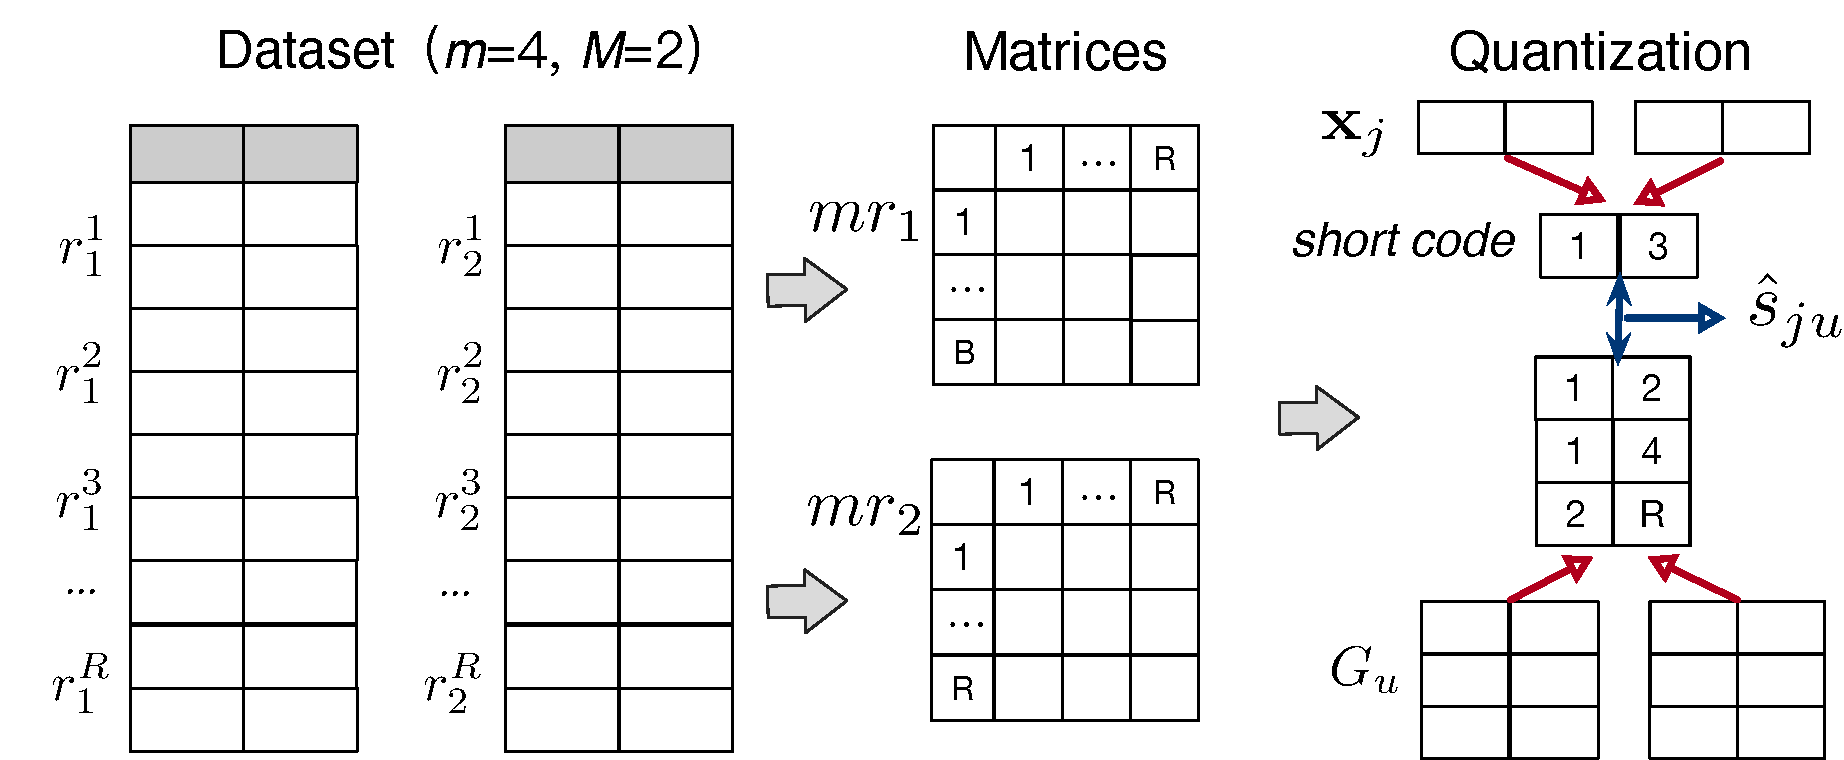
\includegraphics[width=0.7\textwidth]{figs/pq}
   % \vspace{-2.5em}
    \caption{Example of  Quantization-based Method.}
    \label{fig:codebook}
   % \vspace{-1.5em}
\end{figure}



\noindent \textbf{Reducing the number of possible worlds.} Recap that $\mathrm{E}[\min_{c_j\in \hat \core}\hat{s}_{ju}] = \sum_{x=1}^{card(u)} q_x \min_{c_j \in \hat{C}} \hat{s}_{ju}[x]$.
%
 %And the time complexity is $O(KhUL_{\group}L_t)$, where $L_{\group}$ donotes the number of possible worlds of $\group_u$ and $L_t$ denotes the number of possible worlds of a tuple $t$.
 Hence, since each group contains multiple tuples, possibly multiple missing values,  it is expensive to enumerate $card(u)$ possible worlds and  to get the expectation. 
 To address this, similar to the method discussed in
 Section~\ref{subsec:batch},  we can reduce the number ($L$) of possible worlds of each tuple, and just keep several top possible worlds, say $l$, with the highest probabilities. 
%  Next, suppose that there are $b$ tuples with missing values, and thus $3^b$ possible worlds are generated for $G_u \cup \hat{C}$. To achieve further acceleration,   we can  select top-$l_G$ (\eg 3)possible worlds from the $3^b$ ones to compute the expectation. 
\jks{Next, suppose that there are $x+1$ tuples (x tuples in $G_u$ and one tuple in $\hat{C}$) with missing values, and thus $l^{x+1}$ possible worlds are generated for $G_u \cup \hat{C}$. To achieve further acceleration, we can select top-$l_G$ (\eg 3)possible worlds from the $l^x$ ones to compute the expectation.}
 Overall, the time complexity is $O(KhUll_{\group})$, which is much faster than the $O(Khnl^2)$ because $U \ll n$ and $l_G$ is also small. Similarly, the above framework is easy to generalize to the scenario of one batch per iteration, where the only difference is that in the coreset, we have a small batch of tuples with missing values rather than just one, indicating that the number of possible worlds that should be considered increases. However, we can still reduce the possible world number following the above method. \jks{Finally, the time complexity of one batch per iteration is $O(KhUll_{\group}^b)$}
 
 
 % $\sum_{u=1}^U  |\group_u| \times\mathrm{E}[\min_{c_j\in \hat{\core}}\overline{s}_{\gamma(j)u}]$
 
 
 \noindent \textbf{Time complexity analysis.}
 We can sample a small subset to compute the clusters in each subspace, and thus the time complexity of this part can be ignored. 
 %
 Then the matrices can be computed in $O(mR^2)$ and the short codes of $\train$ can be computed in $O(mnR)$. 
 %
 %
 As discussed above,  the largest distance between corresponding codes of  $c_j$ and codes of tuples in $\group_u$ can be computed by $\hat{s}_{ju}^z = \max\limits_{v\in\group_u}mr_z[d_{j}^z][d_v^z]$ in the $z$-th subspace. 
 %
 %
 As $d_j^z$ only takes from $R$ different values $\{1, 2, \dots, R\}$, we can precompute $\max\limits_{v\in\group_u}mr_z[i][d_v^z], i\in[1, R]$ for each $\group_u$, which takes $O(UR^2)$. In this way, we can compute each $\hat{s}_{ju}=\sum_{z=1}^{M}\hat{s}^z_{ju}$ in $O(M)$, and all the upper bounds $\hat{s}_{ju}$, $j\in [1,N]$, $u\in [1,U]$ can be computed in  $O(MnU)$.%, much faster than the $O(mn^2card(u))$.
 
\noindent \textbf{Convergence analysis.}  
Considering the proof in Section~5.3, 
obviously, given a dataset, $\overline{s}_{\gamma(j)u}$ can be bounded (suppose that $\overline{s}_{\gamma(j)u} \leq s_{0}$). Then we have
$\mathrm{E}[\min_{c_j\in \hat{\core}}\overline{s}_{\gamma(j)u}] = \sum_{x=1}^{card(u)} q_x \min_{c_j \in \hat{C}} \overline{s}_{ju}[x] \leq \sum_{x= 1}^{card(u)} q_x * s_{0} = s_{0}$, and thus  $\mathrm{E}[C] = \sum_{u=1}^U  |\group_u| \times\mathrm{E}[\min_{c_j\in \hat{\core}}\overline{s}_{\gamma(j)u}] \leq n * s_{0} = \kappa_1$. And we also have $max_{\hypo \in \vartheta} \Vert \sum_{i=1}^{n} \nabla \fun_{i}(\hypo) - \sum_{j=1}^{\vert \core \vert} w_j \nabla \fun_{\gamma(j)}(\hypo) \Vert \leq \sum\limits_{i=1}^n \min \limits_{c_j\in\core}\lVert \df_i(\hypo) - \df_{\gamma(j)}(\hypo) \rVert \leq \sum\limits_{i=1}^n \min \limits_{c_j\in\core} \dist_{ij}  \leq \kappa_1$.
%Thus, given a coreset $\core$, $\sum\limits_{i=1}^n \min \limits_{c_j\in\core} \dist_{ij}  \leq \sum\limits_{i=1}^n s_{0} \leq n * s_{0} = \kappa_0$.Apparently, we have $\kappa_0 = \kappa_1$. Then, we have $max_{\hypo \in \vartheta} \Vert \sum_{i=1}^{n} \nabla \fun_{i}(\hypo) - \sum_{j=1}^{\vert \core \vert} w_j \nabla \fun_{\gamma(j)}(\hypo) \Vert \leq \sum\limits_{i=1}^n \min \limits_{c_j\in\core}\lVert \df_i(\hypo) - \df_{\gamma(j)}(\hypo) \rVert \leq \sum\limits_{i=1}^n \min \limits_{c_j\in\core}\lVert \dist_{ij} \rVert \leq \kappa_1$. In addition, we use incremental gradient method in Algorithm~\ref{alg:framework}, we have $\Vert \hypo_t - \hypo^{*} \Vert \le \kappa_2$.
Then we can still apply Cauchy-Schwarz inequlity~\cite{strang2006linear} to justify the convergence of the group-based method.
 
 %one simple way to boost efficiency is by minimizing the number of possible worlds. To achieve this, we can intuitively prioritize possible worlds with higher probabilities, allowing us to discard those with lower probabilities without significantly impacting the accuracy of expectation calculations. It's important to note that the probability of each possible world is determined by multiplying the probabilities of incomplete tuples within that world, as these tuples can be considered independent. Hence, we can eliminate possible worlds containing tuples with low probabilities, effectively reducing the overall number of possible worlds in the coreset. 
 
 %For example, we can keep top-$l_\group$(e.g., $l_\group = 3$) possible worlds (\ie 3 different possible worlds of imputations of $\group$ with high probabilities) of a cluster $\group$ and keep top-$l_t$(e.g., $l_t = 3$) possible worlds (\ie 3 different possible worlds of imputations of tuples with high probabilities) of a tuple $t$. The time complexity for computing $\mathrm{E}[t|\core]$ is $O(Ul_{\group}l_t)$ Overall, the time complexity is $O(KhUl_{\group}l_t)$, which is much faster than the $O(Khnl^2)$ because $U \ll n$.
 
 \iffalse

\noindent \textbf{Generalizing to one batch each iteration.}
One tuple per iteration by humans  requires many human iterations.  we propose a trade-off solution that asks the human to impute a small batch of tuples per human iteration.


To be specific, in Algorithm~\ref{}, we introduce an additional parameter: the batch size $b$, which allows for more efficient processing. When $b=1$, Algorithm~\ref{} essentially reverts to the modified Algorithm~\ref{alg:group}, where each tuple is handled individually.Algorithm~\ref{} retains the structure of three loops, yet it diverges in its approach to handling incomplete tuples. Instead of immediately prompting the human for the most beneficial tuple $t^*$ among $T_{sample}$, we simply incorporate $t^*$ into the coreset $\core$ (line~\ref{batch:addcoreset}). Only after accumulating $b$ incomplete tuples do we solicit the human to impute them collectively (lines~\ref{batch:batchenough}-\ref{batch:batchzero}). Subsequently, we compute the weight (line~\ref{batch:weight}), mirroring Algorithm~\ref{alg:group}.

Although this modification reduces the number of human iterations, it elongates the time required to compute $\mathrm{E}[t|\core]$ (line~\ref{batch:loop3}) compared to Algorithm~\ref{alg:framework}. This is due to the increased number of incomplete tuples, resulting in a larger number of potential scenarios to consider. Specifically, the time complexity for computing $\mathrm{E}[t|\core]$ is $O(Ul_{\group}l_t^b)$.

\fi